%#!platex main.tex

\section{Fractal}

\emph{フラクタル}(fractal)は数学者ブノワ・マンデルブロ(Benoit
B. Mandelbrot)が提唱した幾何学の概念である.フラクタル図形と呼ばれる図形
は自己相似性を持ち, 図形のどこを拡大しても全体と同じ形を見ることができる.
図\ref{fig:gasket}は\emph{シェルピンスキーのギャスケット}と呼ばれるフラ
クタル図形である.三角形を一定の法則に基づいて分割していくことで,無限に
続いていく三角形が得られる.その形はどこを拡大しても同様の法則性を持った
図形が得られる.また,自然界の多くの場面でもフラクタル構造をみることがで
きる. 海岸線や, シダ植物などにもフラクタル構造をみることができる. フラク
タルを考えることは自然科学研究の新たなアプローチとしても発展した.

自己相似性を持つ図形はフラクタルという名がつけられる以前から研究されてい
たが, 名が付けられることで, 研究が進むことになった. しかし, こうした図形
達に名が付けられたことに加え, コンピュータの普及により様々なフラクタル図
形を計算, 描画することができるようになり,アートとしても大きく発展した.

フラクタルの特異な形状は多くの人々の興味を引き, アートとしても大きく発展
した. これにはコンピュータの普及も大きく関連しており, コンピュータ文化と
の関連は切り離せない. フラクタルに関するコミュニティとして最大ともいえる
ウェブサイトに, Fractal Forum\footnote{Fractal Forum:
\url{http://www.fractalforums.com/}}がある. この章でこのコミュニティから
生れたフラクタル図形や描画手法は多く, この章で紹介するフラクタルも
Fractal Forumから生れた. これらのフラクタルは数学的な研究対象にならない
ものが多いものの, アートとしては非常に興味を引く形状を持つ.

また,\emph{デモシーン}({\it Demoscene})という文化もフラクタルレンダリン
グと関連が深い.
デモシーンは\emph{デモ}({\it Demo})と呼ばれるリアルタイ
ムにCGグラフィクスや音楽を生成するプログラムを見せ合うコンピューターサブ
カルチャーの一つである.美しいコンピュータグラフィクスを効率よく,さらに
小さなサイズのプログラムで描画することを追求しており, 数式で複雑な形状を
描画できるフラクタルと相性が良い.
また, デモからは様々な最適化手法をみることができる.
 デモシーンに関しては,Demoscene - The
 Art of the Algorithm\footnote{Demoscene - The Art of the Algorithms:
 \url{https://www.youtube.com/watch?v=iRkZcTg1JWU}}というドキュメンタリー
 が詳しい.
著名なデモシーナーのInigo Quilez(iq)は自身のウェブページ\footnote{Inigo
Quilez's webpage: \url{http://iquilezles.org/index.html}}にコンピュータグラフィ
 クスに関する様々な記事をまとめている.
 ここで紹介する手法もまとめられているので, 合せて参考にされたい.

\begin{figure}[htbp]
 \center
 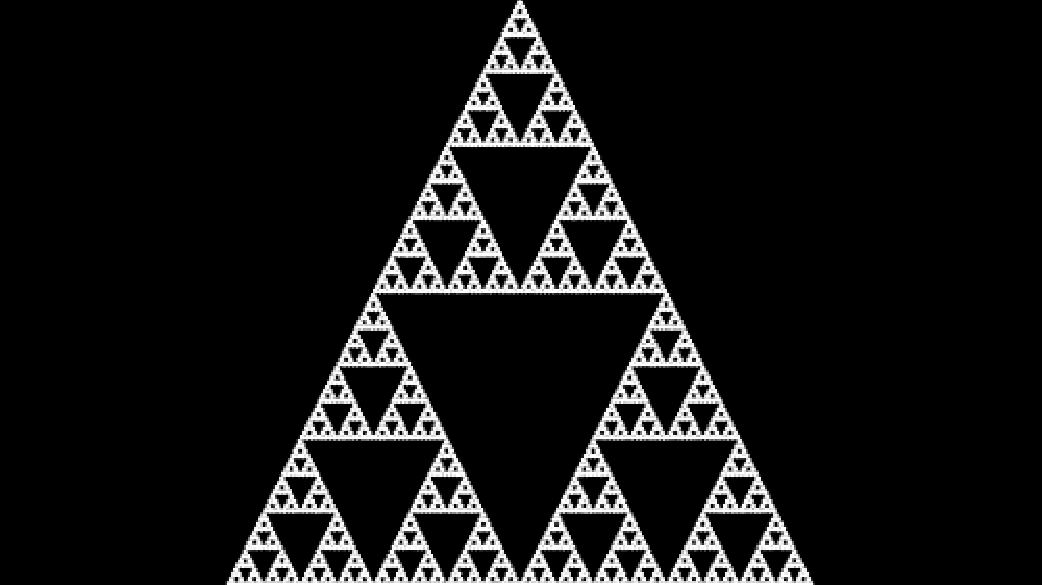
\includegraphics[width=3in, height=3in, keepaspectratio]{../img/fractal/gasket.pdf}
 \caption{Sierpinski gasket}
 \label{fig:gasket}
\end{figure}

\subsection{About Rendering}

この節では,近年よく使われるシェーダを用いたレンダリング手法について触れる.
最近のデモ作品でよく用いられる作品制作手法の1つに\textit{OpenGL Shading
Language(GLSL)}や\textit{High Level Shading Language(HLSL)}の\emph{フラ
グメントシェーダ}(Fragment Shader)を用いるものがある.
フラグメントシェーダは本来,ポリゴンに陰影をつけるために使用され, その処
理はGPUで行なわれる.
GPUは浮動小数演算性能に優れていることに加え,各ピクセルの演算は並列に行
われるため高速である.

この手法では, スクリーンスペースに矩形のポリゴンをレンダリングすることで
\emph{プロシージャル}(\textit{Procedural})に図を描画する.
プロシージャルとは, 数式やアルゴリズムを用いて形状を生成すること等を
指す.
複雑な形状をポリゴンで表現するよりもプログラムの実行サイズを下
げたり, 計算速度を向上させたりすることができるため, デモの, 小さなプログ
ラムサイズでリアルタイムにレンダリングするという目的に適している.
フラクタルはしばしば簡潔なアルゴリズムで複雑な形状を生成するので, デモに
おいてもよく使われる.

アルゴリズム\ref{shaderSample}に擬似コードと図\ref{fig:simpleShader}にレ
ンダリング結果を示した.
このように, ピクセルごとに座標が与えられるので, これを用いてピクセルの色
を決定する.

\begin{algorithm}
 \begin{algorithmic}
\begin{minipage}{0.5\hsize}

 \caption{Sample Shader}
 \label{shaderSample}
  \REQUIRE COORDINATES, resolution
  \STATE uv = COORDINATES / resolution
  \STATE COLOR = Vector3(uv.x uv.y, 1.)
\end{minipage}
 \end{algorithmic}
\end{algorithm}


幾何図形を描く際には多くの場合, 距離関数を用いる.
距離関数は, 図形からの最短距離を返す関数である.
原点中心,半径$r$の円の距離関数は以下のようになる.
\begin{align*}
 f(z) =  length(z) - r
\end{align*}
この関数は円周からの距離を返す.
座標が, 負の距離をもつときに色をつけるような処理を書く
と円を描くことができる.
アルゴリズム\ref{renderCircle}に疑似コードと図\ref{fig:circleShader}にレ
ンダリング結果を示した.
複数の図形を描きたい時は,複数の距離関数を評価し,最も小さな距離を求めれ
ばよい.

また,距離関数は陰関数から近似的に導出することができる.
この手法をDistance Estimationとよぶ.
その式の一つをここで紹介する.
与えられた点$x$に対して, 陰関数$f(x)$が表す零点集合への最短距離を返す近
似関数は微分を用いて以下のように求めることができる.
\begin{align*}
 DistanceFunction(x) \approx \frac{|f(x)|}{|\bigtriangledown f(x)|}
\end{align*}
詳しい導出はiqによるものが詳しい\footnote{distance estimation:
\url{http://iquilezles.org/www/articles/distance/distance.htm}}.

\begin{algorithm}
 \begin{algorithmic}
  \caption{Render circle}
  \label{renderCircle}
  \REQUIRE COORDINATES, resolution
  \STATE p = COORDINATES - (resolution / 2.)
  \STATE distance = length(p) - radius
  \IF{distance $\leq$ 0}
  \STATE COLOR = Vector3(1, 1, 1)
  \ELSE
  \STATE COLOR = Vector3(0, 0, 0)
  \ENDIF
 \end{algorithmic}
\end{algorithm}

 \begin{figure}[htbp]
  \begin{minipage}{0.5\hsize}
   \center
   
\includegraphics[ height=1.5in, keepaspectratio]{../img/fractal/uv.pdf}
   \caption{Simple shader}
   \label{fig:simpleShader}
  \end{minipage}
  \begin{minipage}{0.5\hsize}
   \center
   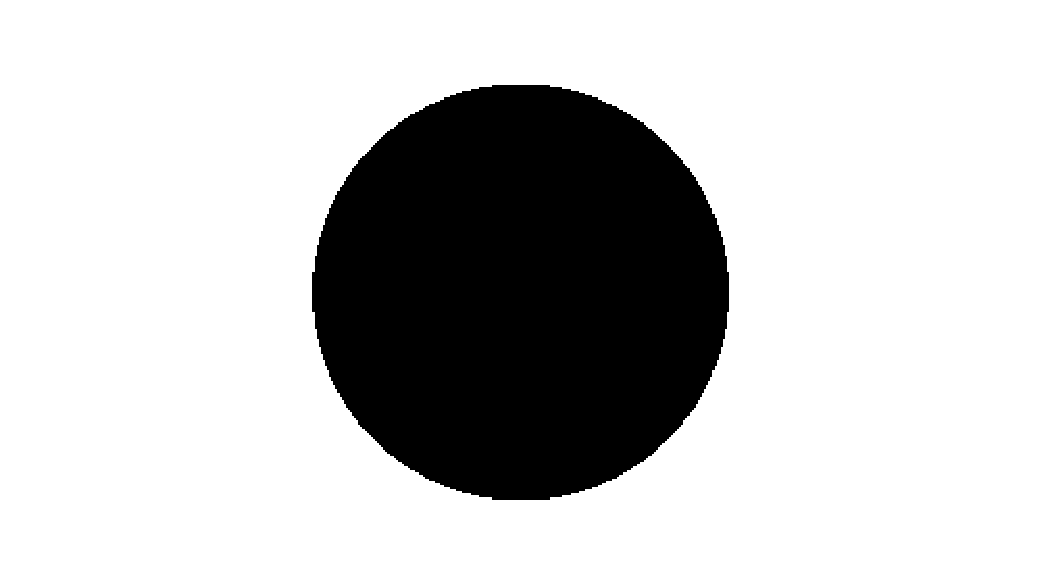
\includegraphics[ height=1.5in, keepaspectratio]{../img/fractal/circle.pdf}
   \caption{Circle}
   \label{fig:circleShader}
  \end{minipage}
 \end{figure}

シェーダで三次元形状を描画する際には\emph{レイトレーシング}({\it Ray
tracing})が用いられる.
レイトレーシングはあらかじめ設定された視点(カメラ)からスクリーンへ
\emph{レイ}({\it Ray})を飛ばし,
その挙動を計算することで物体を描画する手法である.
レイと物体の交差点はレイの方向と位置から代数的に計算することができる.
また,\emph{レイマーチング}({\it Ray marching, Sphere tracing}とも呼ばれ
る)\cite{sphereTracing}という手法を用いることで,距離関数を用いて任意の
三次元形状との交差点を近似的に計算することができる.
物体の形状を代数的に計算することが難しいフラクタル形状のレンダリングを行
う際は,Distance Estimationにより近似的に物体との距離を得てレイマーチン
グと併用することで,高速に描画することができる.

GLSLによるレンダリングや, レイマーチングに関してはdoxasによる
wgld\footnote{wgld: \url{https://wgld.org/d/glsl/}}によくまとまっている.
シェーダを用いたレンダリングはglslsandbox\footnote{glslsandbox:
\url{http://glslsandbox.com/}}やShadertoy\footnote{Shadertoy:
\url{https://www.shadertoy.com/}}といったウェブサービスで手軽に試すこと
ができる.

GPUの計算性能をより汎用的な計算に用いるためのプラットフォームとしてCUDA
やOpenCLが登場している.
これらのプラットフォームを用いることでシェーダではできない複雑な処理を行
うことができるようになり,GPUによる並列演算は機械学習などの分野にも活躍
の場を広げた.
このようにGPUによる演算を画像処理以外の汎用的な用途に用いる技術はGPGPUと
呼ばれている.

\subsection{Escape-time Fractals}
{\it Escape-time Fractals}は複素平面上の点に対して,特定の漸化式を計算し,
その点の軌道の収束,発散を見ることで描画されるフラクタルである.
Escape-time Fractalsで代表的なものが\emph{マンデルブロ集合}({\it
Mandelbrot set})である.
マンデルブロ集合の漸化式は以下のようになる.
\begin{eqnarray*}
 \begin{cases}
  z_{n+1} = z^2_{n} + c \\ z_0 = 0
 \end{cases}
\end{eqnarray*}
$\displaystyle \lim_{x \to \infty} z_n$が無限大に発散しないものをマンデ
ルブロ集合と呼ぶ.図\ref{fig:mandelbrot}における黒い部分がマンデルブロ集合である.
発散と判定されるまでの計算の回数によって色をつけた.
マンデルブロ集合はその単純な式から驚くほど豊富なバリエーションの図を見ることができる.
その他のEscape-time fractalには,\emph{ジュリア集合}({\it Julia set})(図
\ref{fig:julia})や\emph{ファトゥー集合}({\it Fatou set})等がある.

各点における漸化式の計算はお互いに干渉しないので,そのままシェーダでの実
装が可能であるが,先に述べたDistance Estimationを用いることで,エイリア
シングノイズ等を避けてより精細に描画することができる.
これには{\it Green Function}と呼ばれる陰関数を用いる.
導出はiq氏の記事が詳しい\footnote{distance rendering for fractals:
\url{http://iquilezles.org/www/articles/distancefractals/distancefractals.htm}}
.
Green Functionに関しては,マンデルブロ集合に関する詳細な議論となってしま
うので,こちらの論文\cite{mandelbrot}を参考にされたい.

\begin{figure}[htbp]
 \begin{minipage}{0.49\hsize}
  \begin{center}
   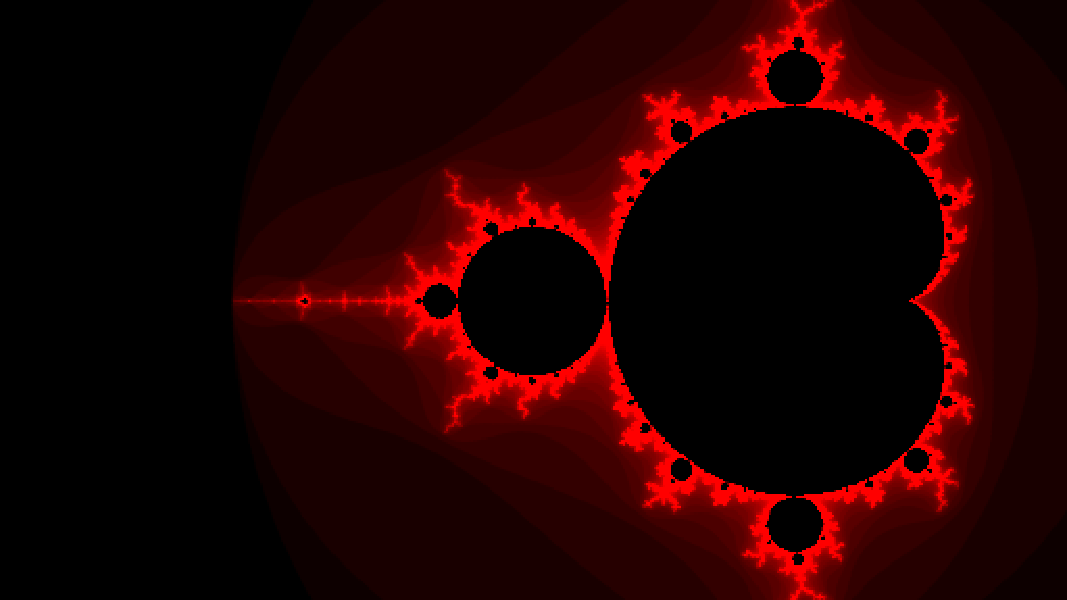
\includegraphics[width=3in, height=3in, keepaspectratio]{../img/fractal/mandelbrot.pdf}
   \caption{Mandelbrot set}
   \label{fig:mandelbrot}
  \end{center}
 \end{minipage}
 \begin{minipage}{0.49\hsize}
     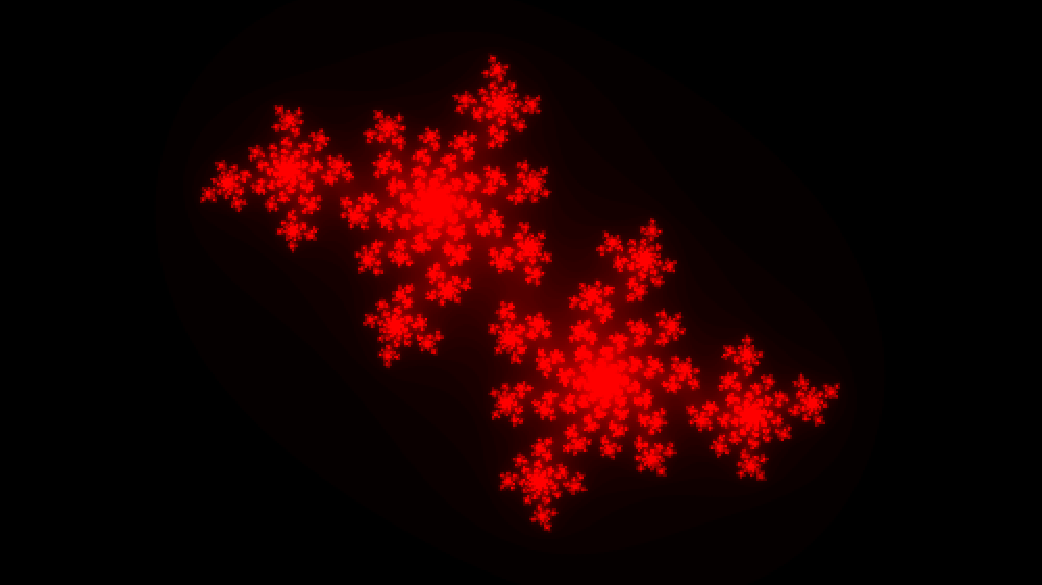
\includegraphics[width=3in, height=3in, keepaspectratio]{../img/fractal/julia.pdf}
   \caption{Julia set}
   \label{fig:julia}
 \end{minipage}
\end{figure}

\subsection{Distance Estimated 3D Fractals}

マンデルブロ集合は数あるフラクタルの中でも複雑な形状を見せるものであった
ので, それを三次元に拡張する方法が考えられてきた.
例えば,ジュリア集合を四元数を用いて,計算したQuaternion Julia 3D
fractal\cite{4djulia}が1989
年には発表されている.
しかし,どの三次元フラクタルもその形状は単純でフラクタルコミュニティの満
足のいくものにはならなかった.

そんな中で, 2003年に発表された阿原・荒木\cite{sphairahedra}による4
次元クライン群の一種である{\it Quasi Fuchsian 3D Fractals}はある程度の複
雑性を持った3次元フラクタルであったため,コミュニティに大きな影響を与え
たと言われている.
このフラクタルに関しては後の章で触れる.

このあたりから, コンピュータのグラフィクス性能が向上し,
2004年にはKeenan CraneがQuaternion JuliaをGPUによってリアルタイムに
描画することに成功した. \footnote{Ray Tracing Quaternion Julia Sets on
the GPU:
\url{https://www.cs.cmu.edu/~kmcrane/Projects/QuaternionJulia/}}.

その後,2009年にマンデルブロ集合をうまく三次元に拡張した{\it
Mandelbulb}の出現を皮切りに,次々と複雑な三次元フラクタルの式が発見され
た.これらもDistance Estimationとレイマーチングを用いることで効率よくレ
ンダリングすることができる.これらのフラクタルはDistance Estimated 3D
Fractalsと呼ばれることが多い.
これらのフラクタルの歴史と実装についてはMikael Hvidtfeldt Christensen氏
のSyntopiaの一連のブログポスト\footnote{Syntopia, Distance Estimated 3D
Fractals:\\ \quad \quad
\url{http://blog.hvidtfeldts.net/index.php/2011/06/distance-estimated-3d-fractals-part-i/}}
によくまとめられている.

これらフラクタルをレンダリングするためのソフトウェアは{\it Mandelbulb
3D}\footnote{Mandelbulb 3D:
\url{http://mandelbulb.com/2014/mandelbulb-3d-mb3d-fractal-rendering-software/}}
や{\it Mandelbulber}\footnote{Mandelbulber:
\url{http://www.mandelbulber.com/}}が有名である.
{\it Fragmentarium}\footnote{Fragmentarium:
\url{http://syntopia.github.io/Fragmentarium/}}はシェーダベースのグラフィ
クスを開発するための環境である.
フラクタルのサンプルコードも豊富で学習に役立つ.
{\it Fractal Lab}\footnote{Fractal Lab:
\url{http://hirnsohle.de/test/fractalLab/}}はブラウザ上でGLSLを用いてフ
ラクタルをレンダリングすることができるWebアプリケーションである.
この章で使われている図のいくつかはFractal Labを用いてレンダリングした.

\subsubsection{Mandelbulb}

マンデルブロ集合を三次元に拡張するにあたって一番の問題は漸化式の意味付けであった.
マンデルブロ集合では複素平面上で計算を行なうため, $z^2$は回転と拡縮, $c$
の加算は点の平行移動を表わし, それによって軌道を見ることができる.
三次元空間の点において, 同様の意味を表わす代数体系のようなものを考える必要があった.
様々なアプローチが考案されたが, 最終的にD.White(twinbee)氏とP.Nylander氏
が開発したMandelbulbが広く知られるようになった.

White氏は球面座標上で漸化式を計算するアプローチを提案
\footnote{\url{http://www.fractalforums.com/3d-fractal-generation/true-3d-mandlebrot-type-fractal/}}
した.
図\ref{fig:mandelbulb2}は$z_{n+1} = z_n^2 + c$を用いてレンダリングした結
果であるが,あまり複雑な形状は現れなかった.
しかし,その後Nylander氏が式を高次の積を扱えるように拡張した.
図\ref{fig:mandelbulb8}は$z_{n+1} = z_n^8 + c $という式でレンダリングさ
れた形状であり,Mandelbulbとして広く知られている.White氏のWebページ
\footnote{Skytopia:
\url{http://www.skytopia.com/project/fractal/mandelbulb.html}}では開発の
詳しい経緯がまとめられている.

Mandelbulbは三次元空間の点に対して漸化式を計算することで形状を得ることも
できるが, 通常はマンデルブロ集合と同様に距離関数を導出し, レイマーチング
を用いてレンダリングする.

\begin{figure}[h!tbp]
 \begin{subfigure}{0.49\hsize}
   \begin{center}
    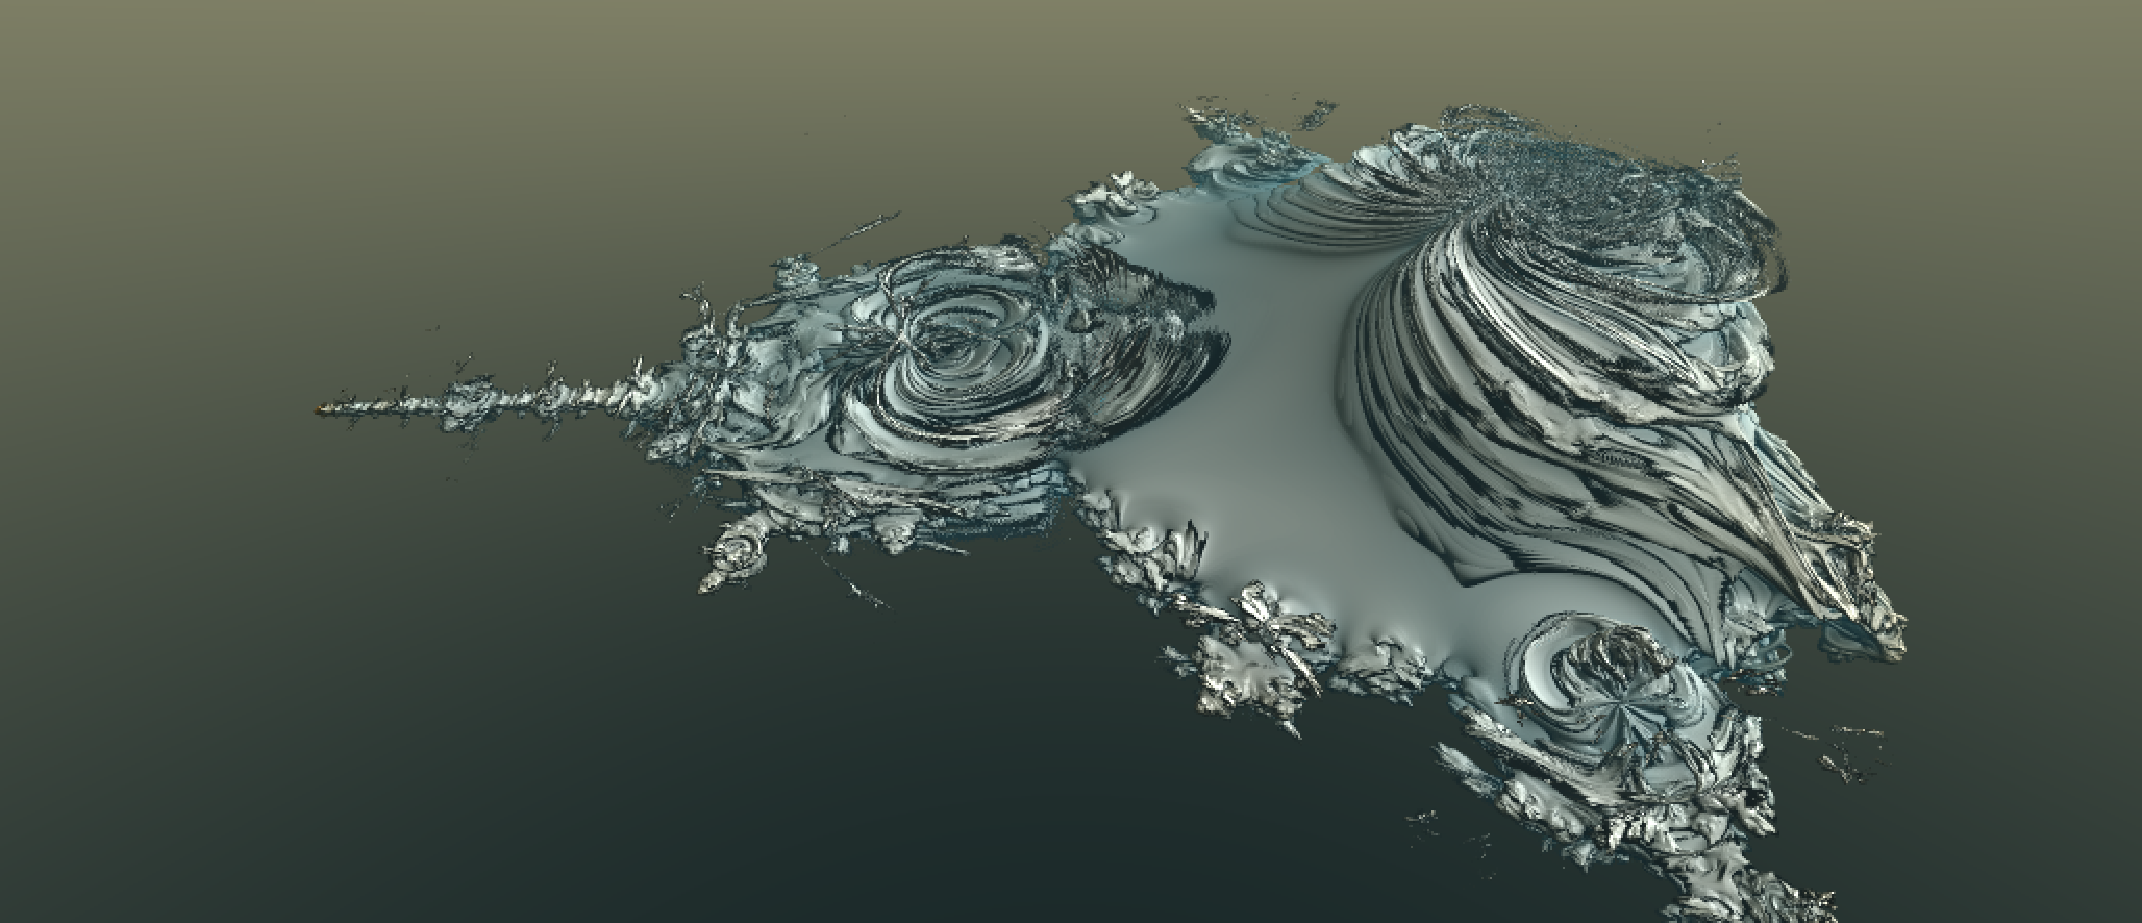
\includegraphics[width=3in, height=3in, keepaspectratio]{../img/fractal/mandelbulb2.pdf}
    \caption{$z_{n + 1} = z_n^2 + c$}
    \label{fig:mandelbulb2}
   \end{center}
 \end{subfigure}
 \hspace*{\fill}
 \begin{subfigure}{0.49\hsize}
   \begin{center}
    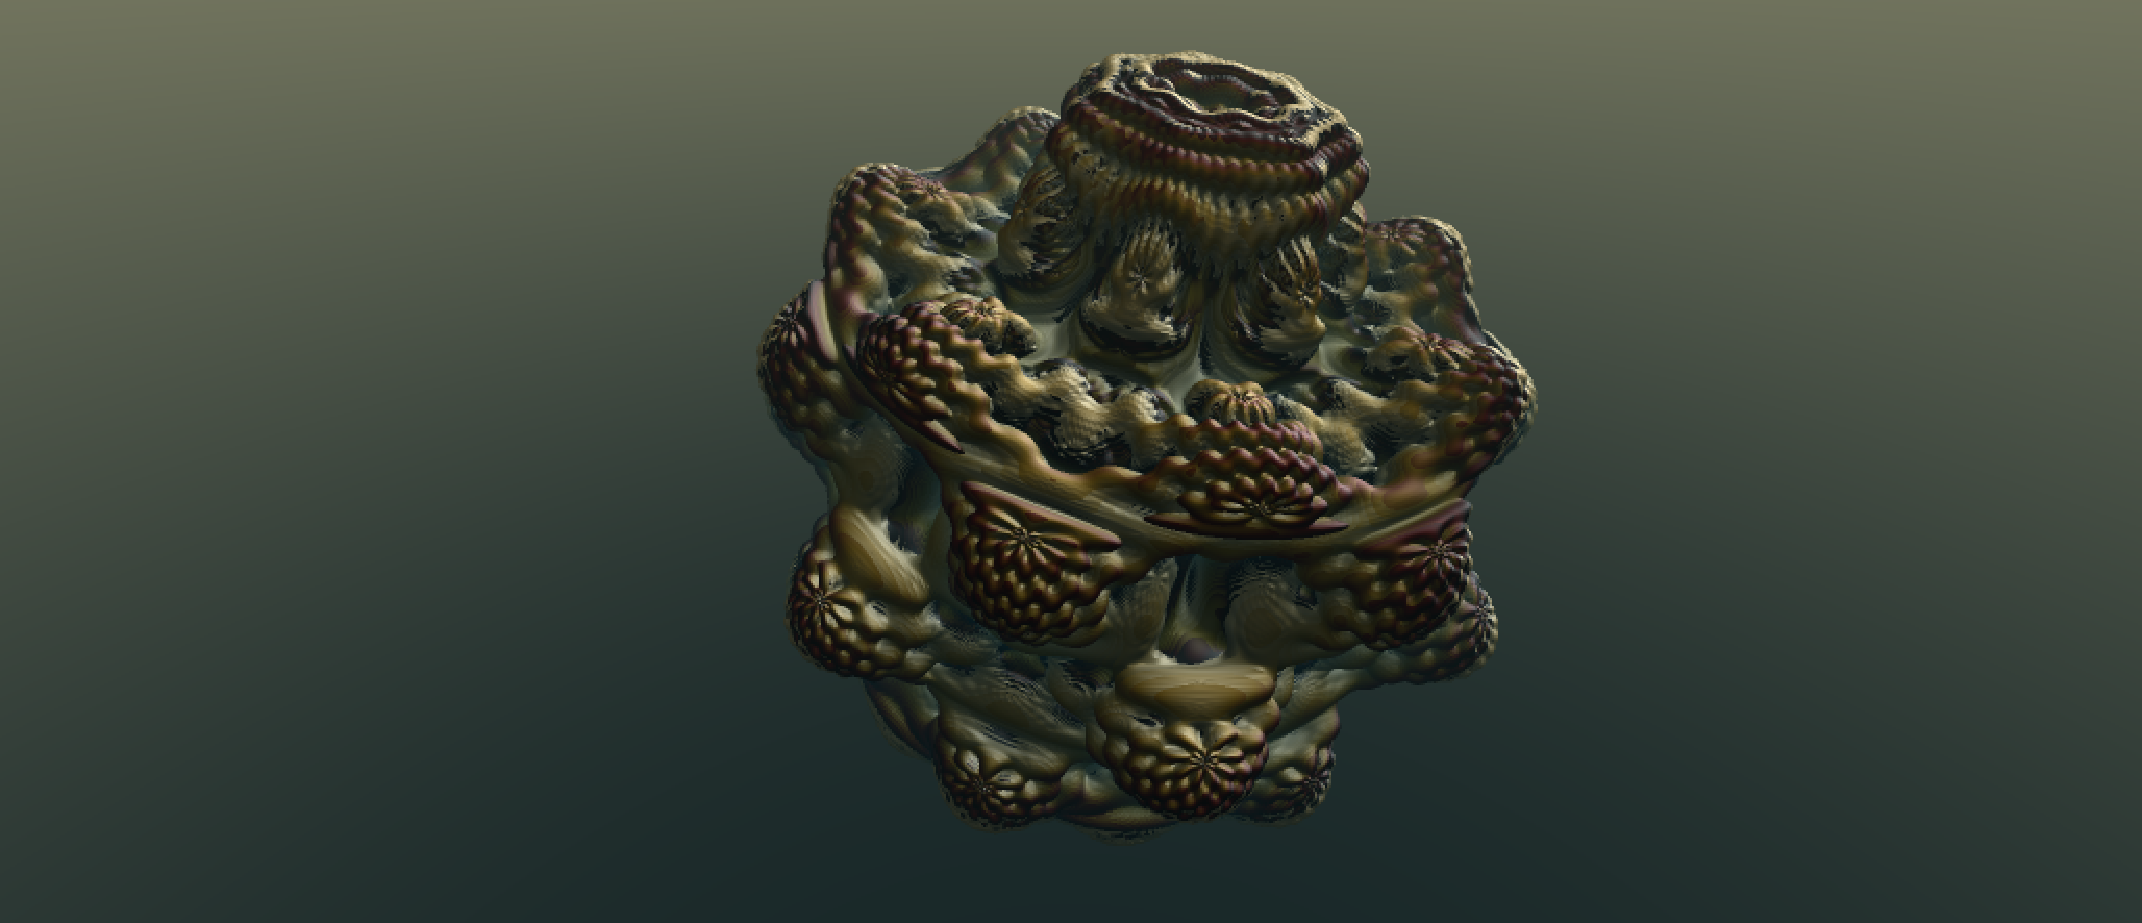
\includegraphics[width=3in, height=3in, keepaspectratio]{../img/fractal/mandelbulb8.pdf}
    \caption{$z_{n+1} = z_n^8 + c$}
    \label{fig:mandelbulb8}
   \end{center}
 \end{subfigure}
 \caption{Mandelbulb rendered by Fractal Lab}
\end{figure}

\subsubsection{Mandelbox}
その後,2010年にTom Lowe氏によって{\it Mandelbox}\footnote{Mandelbox:
\url{https://sites.google.com/site/mandelbox/what-is-a-mandelbox}}が開発
された.
Mandelboxも三次元空間におけるEscape-time fractalである.
漸化式は$z_{n+1} = scale * spherefold(minR, boxfold(z_n)) + c$となる.
ここで, {\it boxfold}は$x=\pm1, y=\pm1, z=\pm1$を頂点にもつ立方体の各面
に対して, 点が外側にある場合にその面に関する反転を行なう操作である.
また, {\it spherefold}は以下の式で定義される.
\begin{eqnarray*}
 spherefold(r, z) = \begin{cases}
                  \frac{z}{r^2} & 0 \le |z| < r \\
                  \frac{z}{|z|^2} & r \le |z|
                 \end{cases}
\end{eqnarray*}
基本は原点中心, 半径1の球に関する反転である.
球の反転は, 中心を無限遠点へ変換するが, Escape-timeアルゴリズムでは中心
付近のほとんどの点が発散と判定されてしまう.
そこでspherefoldでは, 中心付近の点の反転をあらかじめ決めておいた最小の半
径における反転で制限をかけている.

Mandelboxの漸化式の関数には場合分けがある.
そのため,Distance Estimationでは漸化式の微分としてヤコビアンの積を用いる.
式の各操作のたびに, ヤコビアンを累積していき,
最終的な点の原点からの距離ををヤコビアンの積で割ることで距離を近似的に求
めることができる.

\begin{figure}[h!tbp]
 \begin{subfigure}{0.49\hsize}
   \begin{center}
    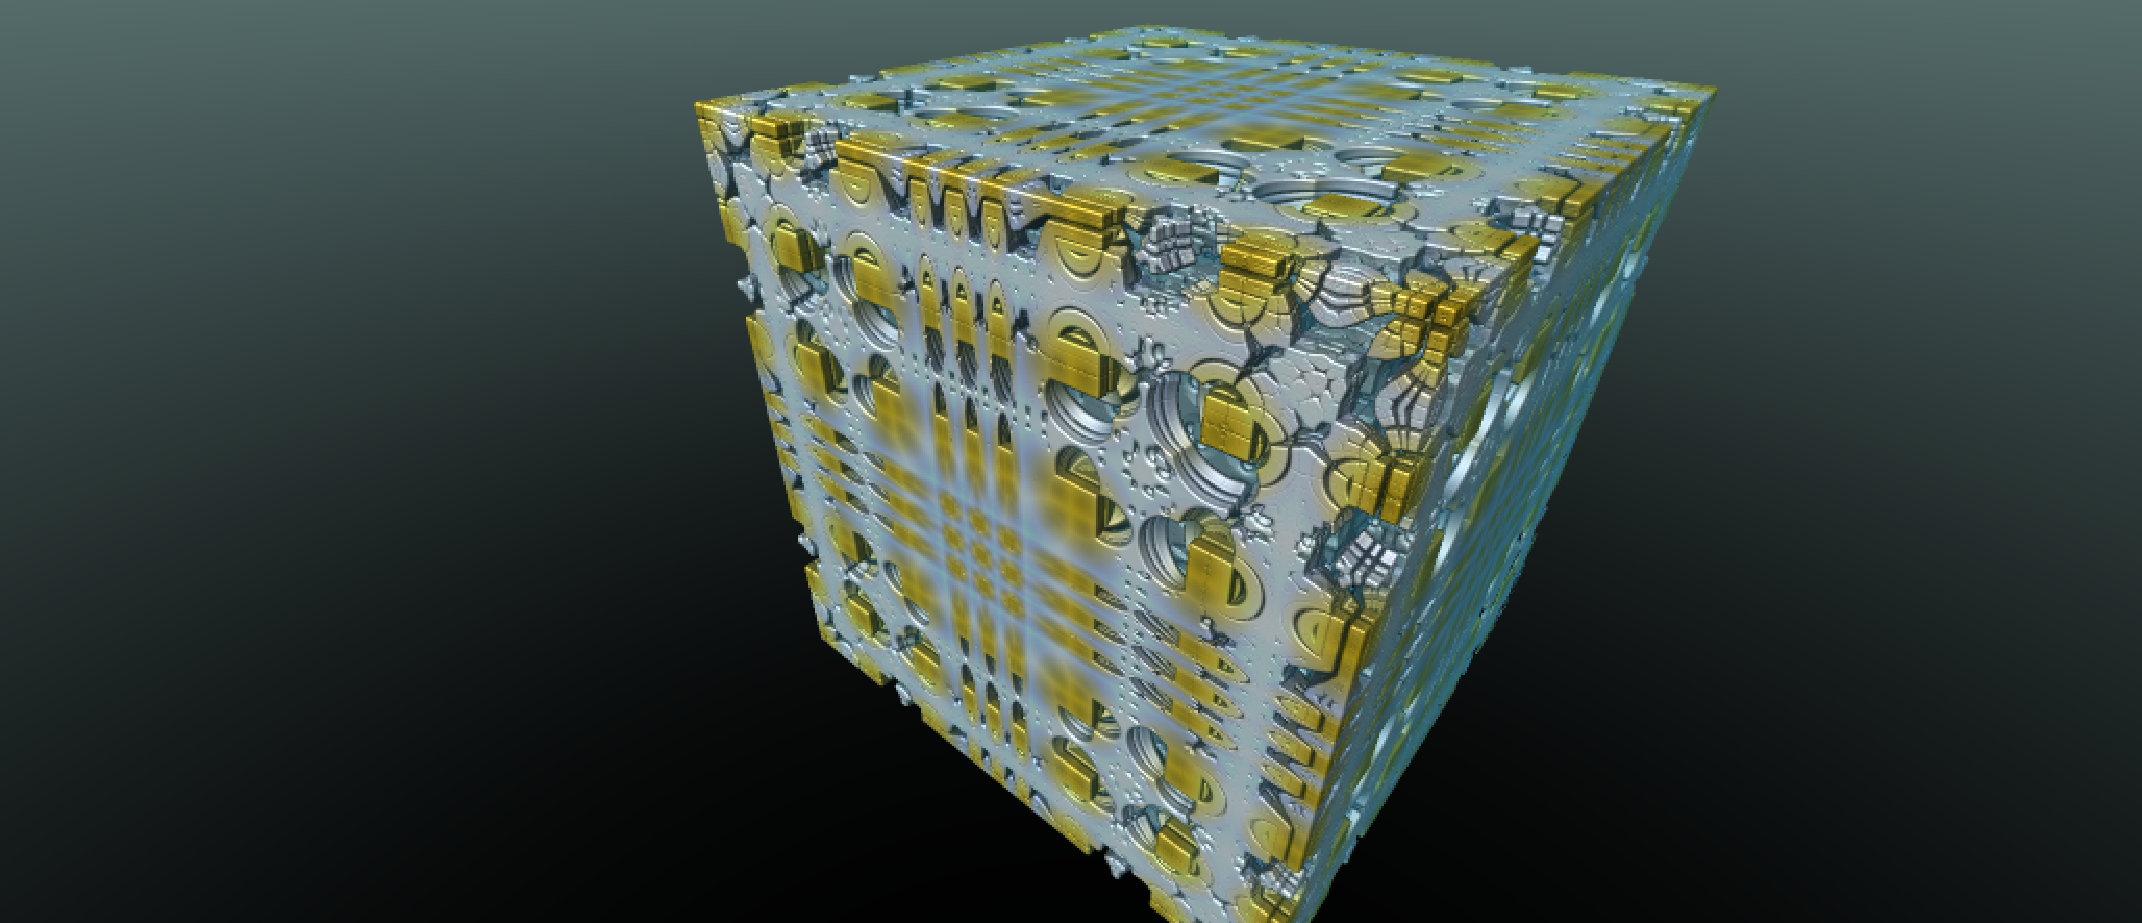
\includegraphics[width=3in, height=3in, keepaspectratio]{../img/fractal/mandelbox.pdf}
    \caption{}
    \label{fig:mandelbox1}
   \end{center}
 \end{subfigure}
 \hspace*{\fill}
 \begin{subfigure}{0.49\hsize}
   \begin{center}
    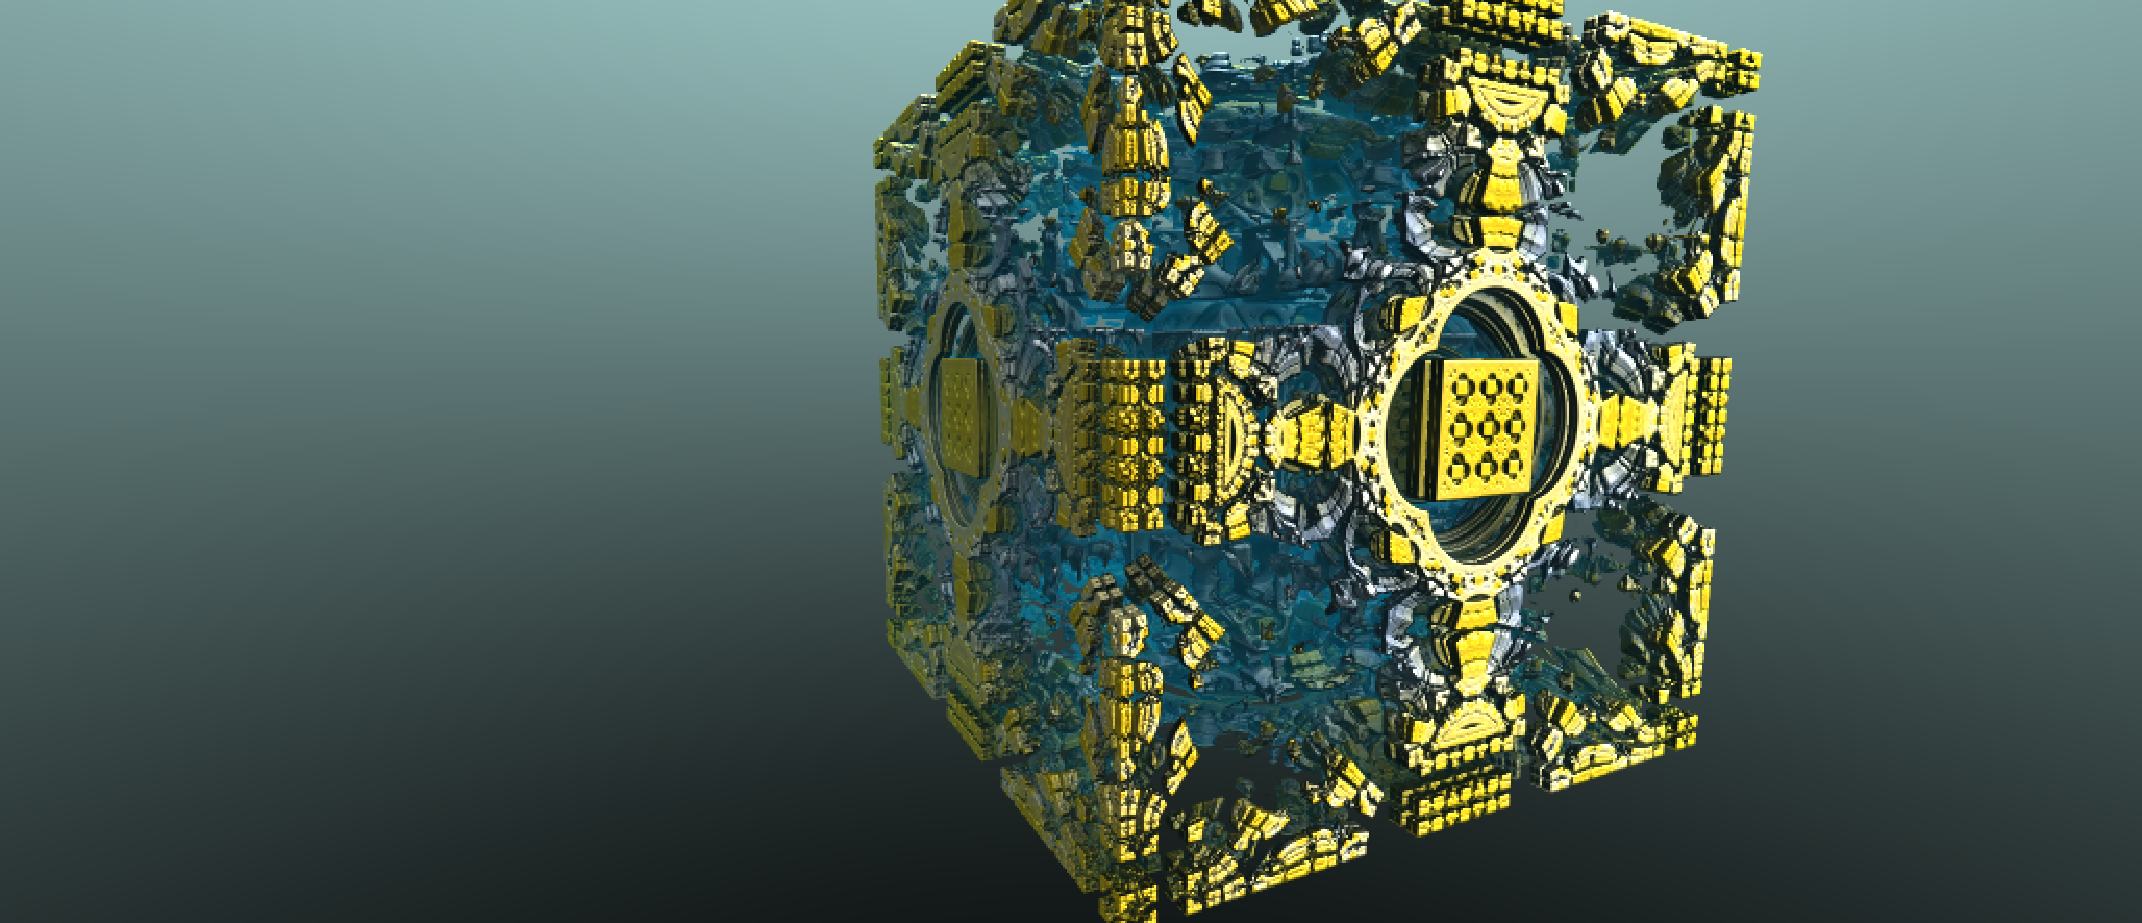
\includegraphics[width=3in, height=3in, keepaspectratio]{../img/fractal/mandelbox2.pdf}
    \caption{}
    \label{fig:mandelbox2}
   \end{center}
 \end{subfigure}
 \caption{Mandelbox rendered by Fractal Lab}
 \label{fig:mandelbox}
\end{figure}


\subsubsection{Pseudo-Kleinian}

Mandelboxの登場以降は漸化式にMandelbulbやMandelboxを含む複数の式を用いた
{\it Hybrid System}によって,様々なフラクタル作品が作られている.
興味深いHybrid Systemの1つに{\it pseudo-kleinian}がある.
これは球の反転に近い操作であるSpherefoldと平行移動と同じような働きをする
boxfoldの組み合わせによってクライン群のような形状が得られる式である.
図はfragmentariumのサンプルスクリプトを用いてレンダリングされた.

\subsection{Coloring by Orbit Trap}

フラクタルのレンダリングにおいて,カラーリングは重要な要素である.
Escape-timeアルゴリズムを用いたフラクタルのカラーリングには,主に{\it
Orbit Trap}とよばれる手法が使われる.
図\ref{fig:mandelbox}のMandelboxもOrbit Trapを用いて色がつけられている.

Orbit trapでは,trapと呼ばれる点や直線などの図形を空間上に置いておき,
trapと漸化式の計算で得られる軌道の点の位置関係から色を付ける方法である.
図\ref{fig:mandelbrotOrbit}はマンデルブロ集合の計算の最中に$z_n$が桃色の
領域に入った点を白く塗った.
桃色の領域に到達するまでの点の軌道を描いたと考えることができる.

また,この方法を応用すると,図\ref{fig:mandelbrotBitmap}のように画像を
trapに用いることで,点の軌道上に画像を張り付けることも可能である.
この手法は特に{\it Bitmap Orbit Trap}とも呼ばれる.

\begin{figure}[htbp]
 \begin{minipage}{0.49\hsize}
  \begin{center}
   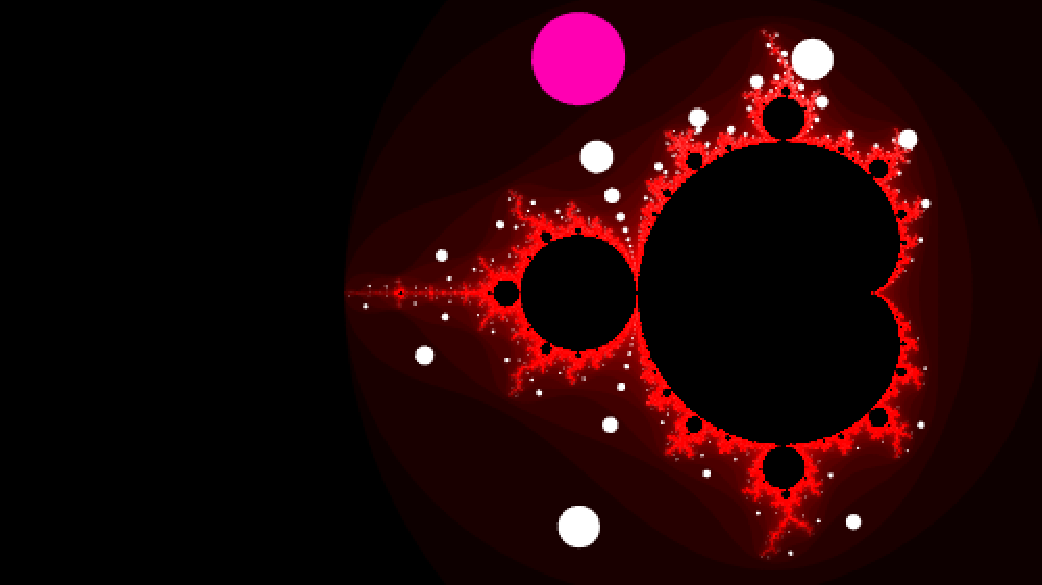
\includegraphics[width=3in, height=3in, keepaspectratio]{../img/fractal/mandelbrot-orbit.pdf}
    \caption{Mandelbrot set}
    \label{fig:mandelbrotOrbit}
  \end{center}
 \end{minipage}
 \begin{minipage}{0.49\hsize}
  \begin{center}
   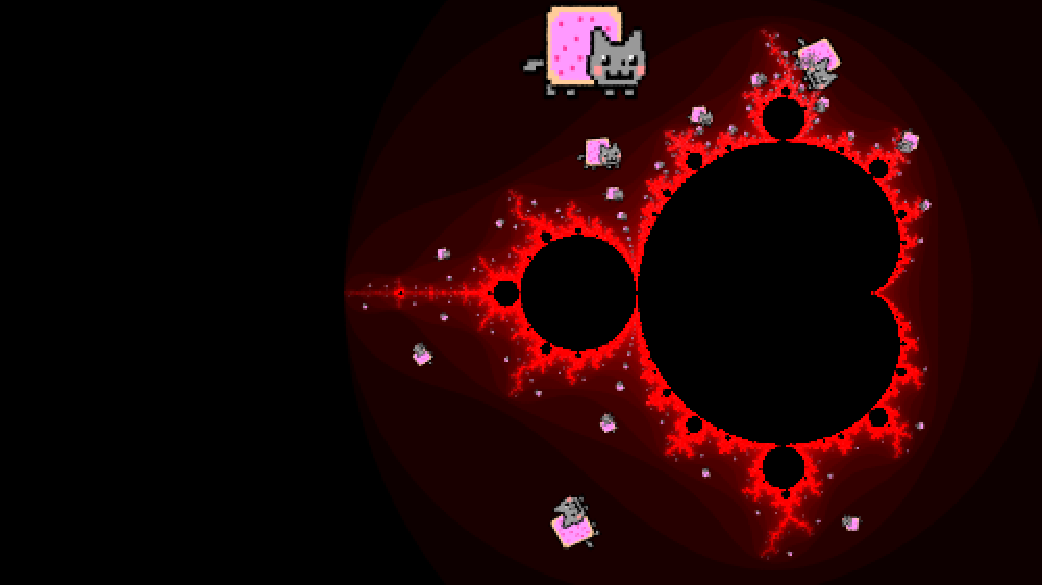
\includegraphics[width=3in, height=3in, keepaspectratio]{../img/fractal/mandelbrot-bitmap.pdf}
   \caption{Mandelbrot set}
   \label{fig:mandelbrotBitmap}
  \end{center}
 \end{minipage}
\end{figure}

\subsection{Other Fractals}

もう一つ有名なアルゴリズムとして,{\it Iterated Function system (IFS)}が
ある.
IFSは平面状の複数の点に様々な関数を適用して,その集積
点をレンダリングするアルゴリズムである.
シェルピンスキーのギャスケットなどもIFSでレンダリングすることができる.
IFSに関する書籍としてFractals Everywhere\cite{fractalsEverywhere}がある.
並列計算による高速化に関して以下の論文にまとめられている
\cite{highPerformanceIFS}\cite{GPUIFS}.

IFSを拡張したフラクタルアートの一種に\emph{フラクタルフレーム}{\it(Fractal
Frame)}\cite{fractalFrame}がある.フラクタルフレームはIFS
に用いる関数にメビウス変換などの非線形変換を用い,美しくレンダリングされ
るようにカラーリング等が工夫されている.

他にも様々なアルゴリズムが存在するが,今回は後述するクライン群のレンダリ
ングには関連してこないので触れない.
マンデルブロ自身の著作\cite{fractal}では種々のフラクタルについて網羅的に
まとめられている.
